\section{Evaluation}\label{sec:eval}

\name{} argues for eschewing standalone orchestrators and, instead, building
application-level orchestration on unmodified serverless infrastructure using
FaaS schedulers and consistent data stores. In this section, we evaluate how
well application-level orchestration performs, reduces costs, and improves
application flexibility. In particular, we focus our performance evaluation on
whether decentralization comes at a reasonable overhead compared with
standalone orchestrators.

Specifically, we answer the following questions:

\begin{enumerate}

  \item What overhead does \name{} incur in end-to-end latency and what are
   the sources of \name{'s} overheads?

  \item How much does it cost to run applications with \name{} and what are
   the sources of costs compared with Step Functions?

  \item How well does \name{} support applications that Step Functions cannot
   support well?

\end{enumerate}

Though we evaluate the applications running on both AWS and Google Cloud, we
focus our discussion on our AWS implementation with Lambda and DynamoDB,
because it runs on the same serverless infrastructure as Step Functions.

\subsection{Experimental setup}

We run all experiments on AWS with Lambda and DynamoDB, and on Google Cloud
with Cloud Functions and Firestore. All services are in the same region
(\texttt{us-west-1} on AWS and \texttt{us-central-1} on Google Cloud). All
functions are configured with 128MB of memory except for ExCamera where we use
3GB of memory to replicate the setup in the original paper~\cite {excamera,
gg-atc}. DynamoDB uses the on-demand provisioning option that charges per-read
and per-write~\cite {dynamodb-pricing}. To avoid performance artifacts related
to cold-starts, we ensure functions are warm by running each experiment
several times before taking measurements.

All but one application were originally written as Step Function state
machines. For Step Function experiments, we ran them directly with the
``Standard'' configuration~\cite{aws-step-functions-standard-vs-express},
which provides similarly strong execution guarantees as
\name{}~\cite{aws-step-functions-exec-gntee}. For \name{} experiments, we
first compiled the Step Functions definitions to \name{} IR, linked the
functions with the \name{} runtime library and finally executed them as
lambdas or Google Cloud functions. The notable exception is our \name{} and
Step Functions implementations of ExCamera, which differ due to a limitation
in the Amazon State Language. As a result, the more efficient \name {}
implementation is written directly in \name{} IR instead of compiled from the
Step Functions definition (\S~\ref{sec:eval:excamera}).

\subsection{Performance}\label{sec:eval:micro}

\name{}'s performance overhead results from the \name{} runtime logic run in
each function as well as API calls to data stores and FaaS engines. We
characterize these overheads by measuring the latency to execute various
patterns consists of \texttt{noop} functions as well as end-to-end performance
of real applications. Overall we find that \name{} performs comparably or
significantly better than Step Functions in most cases owing to higher
parallelism and a more expressive orchestration language, with modest slow
downs in the remaining cases due to implementation deficiencies.

\subsubsection{Chaining}\label{sec:eval:chain}

\begin{figure}[t]
  \centering
  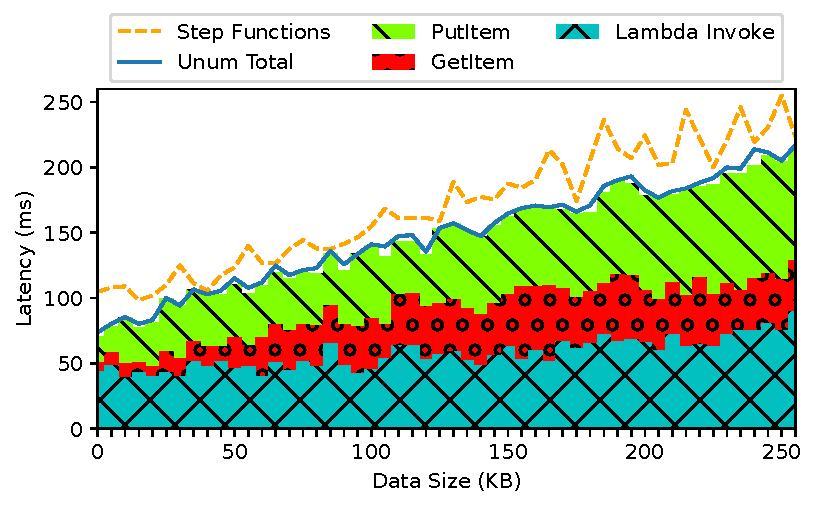
\includegraphics[width=\columnwidth]{figures/TotalAdditionalLatencyNBreakdown.pdf}
  \caption{An orchestrator incurs a latency on each transition between
functions. \name{}'s overhead is due to storage operations to ensure
exactly-one-result semantics, Lambda invocation API overhead to enqueue the
next function to run, and additional \name{} runtime code in the function
instance itself for the orchestration logic.}
  \label{fig:single-transition-latency-breakdown}
\end{figure}

For the simple chaining pattern, the \name{} runtime performs a storage read to
check whether a checkpoint already exists, a storage write to checkpoint the
function's result, and an asynchronous function invocation to initiate the next
function in the chain.

Figure~\ref{fig:single-transition-latency-breakdown} shows time to perform each
of these operations for different result sizes. As expected, storage operations
are slower when checkpointed results are larger, but the total overhead from the
\name{} runtime operations is consistently lower than an equivalent Step
Function transition.

\amit{We can keep Figure~\ref{fig:chainmicrolatency} and explain briefly that this
basically confirms the thing, \emph{but} for that to be the case, it should be
the case that the difference between Step Functions and \name{} increases by
50ms for each additional link in the chain. Is this the case? Otherwise, I
think we can elide this figure.}

The \name{} implementation of the IoT pipeline application benefits from this
difference, with the \name{} version running 1.9x faster than the Step Functions
version (Table~\ref{table:macro}).

\subsubsection{Fan-out and fan-in}\label{sec:eval:fan-out}

\begin{figure}[t]
  \centering
  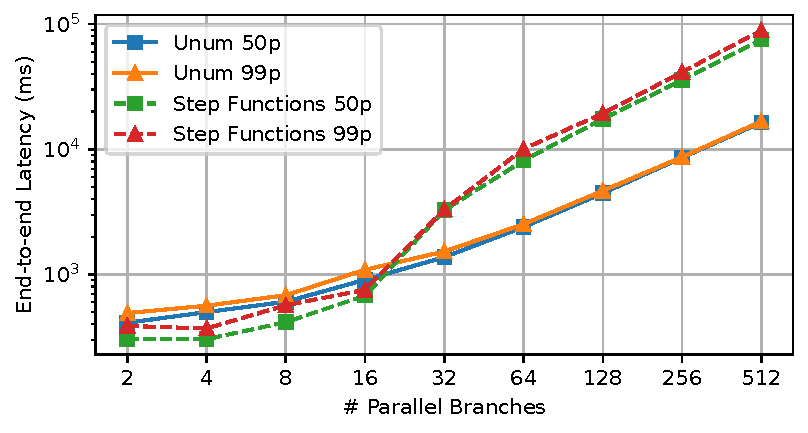
\includegraphics[width=\columnwidth]{figures/MapMicroLatency.pdf}
  \caption{End-to-end latency of a fan-out and fan-in pattern with increasing
branching degree. \name{} is slower at lower branching degrees but significantly
outperform Step Functions at moderate and high branching degree.}
  \label{fig:mapmicrolatency}
\end{figure}

Fan-out requires the same number of storage operations as chaining and similar
orchestration logic, but the \name{} runtime performs an additional asynchronous
invocation at the source function for each branch. For fan-in patterns, each
source branch performs an additional storage read to determine if it is the
final branch to execute, and only the final branch performs the asynchronous
invocation of the target function.

\amit{Why does \name{}'s latency grow at all in \ref{fig:mapmicrolatency}? If it
can do all branches in parallel, shouldn't latency remain roughly constant?}
\dhl{They are not. map invokes each branch in sequence. This is the reason for
unum's worse performance.}

Figure~\ref{fig:mapmicrolatency} shows the latency of a fan-out followed by a
fan-in at varying branching degrees for both \name{} and Step Functions. At
low branching degree, \name{} incurs a modest overhead (up to 200ms) relative
to Step Functions. We believe this is mostly due to our implementation
initiating each branch invocation sequentially. However, at higher branching
degrees (as low as 20 branches), Step Functions limits the number of
outstanding fan-out branches~\cite{aws-step-functions-map-state} while
\name{} is limited only by Lambda's scalability, resulting in over 4x lower
latency with 512 branches.

These differences manifest in real workloads as well. Wordcount is highly
parallel (with 262 parallel mappers and 250 reducers) and performs over 2x
faster on \name{} than on Step Functions (Table~\ref{table:macro}).

Although it may not be the case that standalone orchestrators fundamentally
have to impose limits on the number of outstanding function invocations, this
example shows that it is at least not trivial to ameliorate the constraint. On
the other hand, as a library, \name{} is free from the need to design and
implement yet-another service that supports parallel applications well, but
can instead provide as much parallelism as FaaS schedulers and data stores
permit. FaaS schedulers and data stores already support highly-parallel
applications well, and \name{}’s performance will improve automatically when
these underlying services further improve.

\subsection{Cost}

\begin{table*}[t]
  \centering
  \begin{tabular}{|l|rrr|rrr|}
\hline
                         & \multicolumn{3}{c|}{\textbf{Latency (seconds)}}                    & \multicolumn{3}{c|}{\textbf{Costs (\$ per 1 mil. executions)}} \\ \hline
\textbf{App} &
  \multicolumn{1}{c|}{\textit{Unum-aws}} &
  \multicolumn{1}{l|}{\textit{Unum-gcloud}} &
  \multicolumn{1}{l|}{\textit{Step Functions}} &
  \multicolumn{1}{c|}{\textit{Unum-aws}} &
  \multicolumn{1}{l|}{\textit{Unum-gcloud}} &
  \multicolumn{1}{l|}{\textit{Step Functions}} \\ \hline
\textit{IoT Pipeline}    & \multicolumn{1}{r|}{0.12}   & \multicolumn{1}{r|}{0.81}   & 0.23   & \multicolumn{1}{r|}{\$12.38}             & \multicolumn{1}{r|}{\$6.3}         & \$112.02            \\ \hline
\textit{Text Processing} & \multicolumn{1}{r|}{0.52}   & \multicolumn{1}{r|}{3.56}   & 0.55   & \multicolumn{1}{r|}{\$60.42}             & \multicolumn{1}{r|}{\$31.7}        & \$225.29            \\ \hline
\textit{Wordcount}       & \multicolumn{1}{r|}{408.88} & \multicolumn{1}{r|}{484.12} & 898.56 & \multicolumn{1}{r|}{\$13,433.67}         & \multicolumn{1}{r|}{\$11,727.3}    & \$18,141.19         \\ \hline
\textit{ExCamera}        & \multicolumn{1}{r|}{84.52}  & \multicolumn{1}{r|}{122.63} & 98.42  & \multicolumn{1}{r|}{\$62,684.29}         & \multicolumn{1}{r|}{\$51,617.2}    & \$114,633.13        \\ \hline
\end{tabular}
  \caption{Application latency and costs comparison between \name{} and Step
    Functions. Running applications on \name{} is 1.35x to 9x cheaper than
    on Step Functions. Furthermore, \name{} is faster than Step Functions
    especially for workflows with high degrees of parallelism.}
  \label{table:macro}
\end{table*}

\begin{figure}[t!]
    \centering
    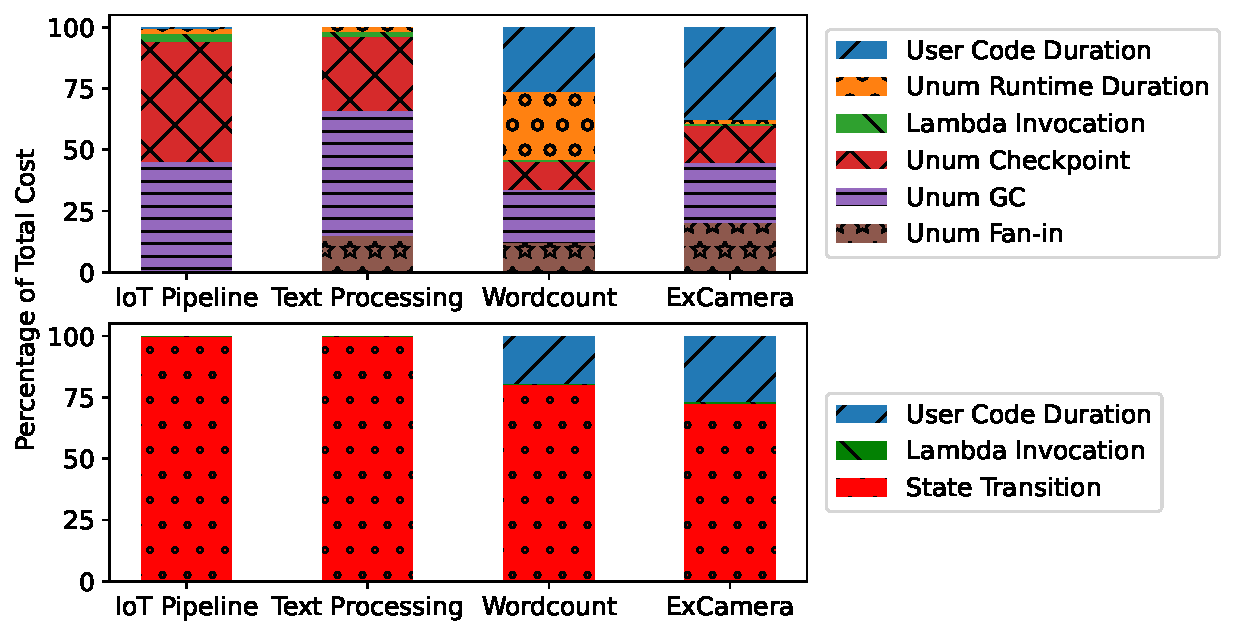
\includegraphics[width=\columnwidth]{figures/AppCostBreakdown.pdf}
    \caption{Step Functions state transitions dominate the total costs for all
    applications (99.5\% in IoT Pipeline, 99.4\% in Text Processing, 80.0\% in
    Wordcount, 72.2\% in ExCamera). While \name{} runtime cost is also the
    majority, it accounts for a smaller portion of the overall costs (95.7\%
    in IoT Pipeline, 97.8\% in Text Processing, 72.5\%
    in Wordcount and 61.0\% in ExCamera).}
    \label{fig:cost-breakdown}
\end{figure}

One of the main attractions of building applications on serverless platforms
is fine-grained and often lower cost. In particular, because resources are
easy to reclaim, applications are charged only for resources used to respond
to actual events. Thus, the \emph{cost} of orchestration matters as well as
performance.

The source of costs for \name{} and Step Functions is quite different. Step
Functions imposes a cost to developers for each workflow
transition~\cite{aws-step-functions-pricing}, such as each branch in a
fan-out. This abstracts the underlying, likely shared, costs to run the Step
Functions servers, persist states and checkpoint data. Conversely, \name{}
incurs costs directly from those services. In particular, compute resources
for executing orchestration logic is charged per-millisecond such as Lambda
runtime cost~\cite{aws-lambda-pricing} and storage for persisting states is
charged per read and write such as DynamoDB reads and
writes~\cite{dynamodb-pricing}.

On AWS, \name{} is much cheaper than Step Functions---AWS's native
orchestrator. For a basic transition in a chaining pattern, Step Functions
charges \$27.9 per 1 million such transitions. On the other hand,
\name{} costs, for 1 million transitions, (1) \$0.42 for $\sim$200ms extra
Lambda runtime to execute orchestration library code, (2) \$2.79 for 1
DynamoDB write to checkpoint, (3) \$0.279 for 1 DynamoDB read to check
checkpoint existence, and (4) \$2.79 for 1 DynamoDB write to garbage collect
the checkpoint. In total, a basic transition in \name{} is about 4.4x cheaper
than the provider-hosted orchestrator on the same platform (\$27.9 vs
\$6.279).

Table~\ref{table:macro} shows the cost to run each of the applications we
implemented based on public pricing information for AWS in the
\texttt{us-west-1} region using \name{} and Step Functions. \name{} is
consistently, and up to 9x, cheaper than Step Functions for the applications
we tested.

Figure~\ref{fig:cost-breakdown} shows the cost to run each application using
\name{} broken down to each component: data store costs for writing and
reading checkpoints, data store costs for writing coordination sets, data
store costs for deleting checkpoints and writing coordination sets for garbage
collection, Lambda invocation, and Lambda CPU-time for both the \name{}
runtime and user function. Storage costs, using DynamoDB, are the largest
portion of overall cost and costs for writing to DynamoDB is the
majority\footnote{Writes in DynamoDB cost about an order-of-magnitude more
than reads}. This includes writing checkpoints, writing to coordination set
(either for fan-in for garbage collection) and deleting checkpoints for
garbage collection.

Of course, developer-facing pricing is only a proxy for \emph{actual} costs of
hardware and human resources. However, it is clear that, in practice,
\name{}'s costs are reasonable and, in fact, often lower than Step Functions.
This suggests that at least applications that currently run on Step Functions
could afford to run using \name{} instead.

Furthermore, services that \name{} builds on---FaaS schedulers and data
stores---are core multi-tenant services that likely multiplex over a larger
audience of applications than orchestrators for greater economies of scales.
These services typically have enjoyed long periods of improvement already to
make them efficient. \name{}'s design obviates the need to host yet-another
service which frees up resources such that providers can focus on fewer core
services in their serverless infrastructure.

Moreover, \name{} automatically benefits from improvements to the underlying
infrastructure and pricing schemes. For example, Azure's Cosmos DB provides
similar performance and consistency guarantees to DynamoDB but charges 5x less
to perform a write operation (the dominant cost of \name{}'s data store
operations).

\subsection{Case Study: ExCamera}\label{sec:eval:excamera}

\begin{figure}[t!]
    \centering
    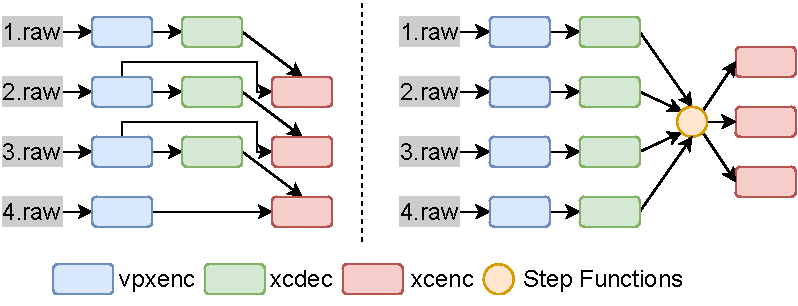
\includegraphics[width=\columnwidth]{figures/ExCameraPattern.pdf}
    \caption{\name{} ExCamera replicates the application logic from gg and mu
     where the re-encode stage (xcenc) of a branch can start immediately when
     the previous branch completes decoding (xcdec) and my own branch
     completes the initial encoding (vpxenc). Step Functions provides a Map
     pattern~\cite{aws-step-functions-map-state} for parallel workloads.
     However, branches in Map must be identical and Map does not support data
     dependencies between branches. As a result, to ensure previous branches'
     xcdec have completed, all branches must first finish and fan-in to Step
     Functions before starting the xcenc step, essentially serializing the
     stage.}
    \label{fig:excamera-pattern}
\end{figure}

\begin{table}
  \centering
  \begin{tabular}{|r|r|}
    \hline
    \textbf{ExCamera Implementation} & \textbf{Latency (seconds)} \\ \hline
    Original        & 76                         \\ \hline
    \name{}-aws & 84                         \\ \hline
    gg                       & 90                         \\ \hline
    Step Functions & 98                         \\ \hline
  \end{tabular}
  \caption{ExCamera performance. \name{} is 7.1\% faster than
gg~\cite{gg-atc} and 10.5\% slower than the hand-optimized implementation.}
  \label{table:excamera}
\end{table}

ExCamera~\mbox{\cite{excamera}} is a video-processing application designed to
take advantage of high burst-scalability on Lambda using custom orchestration.
We compare our \name{} implementation with three others: (1) the original
hand-optimized ExCamera using the mu framework, (2) an implementation using a
generalized orchestrator (gg) by the same authors, and (3) an optimized Step
Functions implementation we wrote.

Both gg and mu employ standalone orchestrators to proxy inter-function
communications, store application states and invoke lambdas. However, mu uses
a fleet of long-running identical lambdas where all application code is
co-located and raw video chunks are pre-loaded, whereas gg lambdas are
event-driven, task-specific and cannot leverage pre-loading. The application
logic, though, is identical for gg ExCamera and mu ExCamera. \name{}'s
ExCamera replicates the application logic from gg and mu. However, the Step
Functions ExCamera implementation must serialize the encode and re-encode
stages because Step Function's Map pattern requires all concurrent branches to
complete before any fan-in starts (Figure~\ref {fig:excamera-pattern}).

\subsubsection{Performance}

Using the same experimental setup as the prior work (i.e., encoding the first
888 chunks of the \texttt{sintel-4k}~\mbox{\cite{sintel}} video using 16
chunks per batch and Lambdas configured with 3GB of memory), \name{} is 7.1\%
faster than gg~\mbox{\cite{gg-atc}} and 10.5\% slower than the original,
hand-optimized ExCamera (Table~\ref{table:excamera}). The original authors
attributes the slower performance of gg ExCamera to the lack of pre-loading
which is likely also the reason for \name{}'s slower performance.

But different from gg, \name{} executes orchestration in a decentralized
manner while gg has a standalone coordinator on EC2. The reduced number of
network communications likely explains why \name{} is slightly faster.

Comparing with Step Functions, \name{}'s design allows the flexibility to
implement ExCamera's original application pattern where tasks start as soon as
their input data becomes available, whereas the Step Functions implementation
had to use the less-efficient Map pattern without the flexibility to add new
orchestration patterns easily. As a result, the \name{} ExCamera enables more
parallelism between branches and is 16.7\% faster than Step Functions.

\subsubsection{Cost}

Unlike \name{}, neither gg nor mu aimed to reduce the cost of running
serverless applications and neither discussed costs in detail. Nevertheless,
there are several important factors in comparing \name{} with gg and mu in
relation to costs.

First, similar to Step Functions, gg and mu both rely on standalone
orchestrators. Thus, the fundamental costs difference is also similar, namely
\name{}'s use of storage vs gg's and mu's use of VMs. mu's orchestrator
consists of a coordinator server as well as a rendezvous
server~\cite{excamera}, while gg's only has a coordinator
server~\cite{gg-atc}. In the mu authors' experiments, they used a 64-core VM
(\texttt{m4.16xlarge}) as the rendezvous server. Neither mu nor gg specified
the instance type of its coordinator server. However, the cost of the
rendezvous server, at the time of writing, is \$3.20 per hour, or
approximately \$2352 per month.

Furthermore, standalone orchestrators must separately consider fault-tolerance
in case of orchestrator failures. Most commonly, fault-tolerance is achieved
by running multiple coordinating instances (replicas) of the service. As a
result, production deployments of mu and gg would likely cost more.

Lastly, deploying an orchestrator per application or per user limits the
ability to amortize costs through multi-tenancy. A provider-hosted
orchestrator, such as Step Functions, can achieve larger economies of scale by
serving many users concurrently with a single deployment.
